\documentclass{article}
\usepackage[utf8]{inputenc}
\usepackage[margin=1in]{geometry}
\usepackage{graphicx}
\usepackage{amsthm, amsmath, amssymb}
\usepackage[loose,nice]{units} %replace "nice" by "ugly" for units in upright fractions
\usepackage{mathrsfs}
\usepackage{wasysym}
\usepackage{faktor}
\usepackage{xcolor}
\usepackage{hyperref}
\usepackage[normalem]{ulem}
\usepackage[shortlabels]{enumitem}
\usepackage[mathscr]{euscript}
\usepackage{mathtools}



\numberwithin{equation}{subsection}

\newtheorem{theorem}{Theorem}[subsection]
\newtheorem{proposition}{Proposition}[subsection]
\newtheorem{lemma}{Lemma}[subsection]

\theoremstyle{definition}
\newtheorem{definition}{Definition}[subsection]


\DeclareMathOperator{\img}{im}
\DeclareMathOperator{\Aut}{Aut}
\DeclareMathOperator{\GL}{GL}
\DeclareMathOperator{\Char}{char}
\DeclareMathOperator{\End}{End}
\DeclareMathOperator{\Hom}{Hom}
\DeclareMathOperator{\Der}{Der}
\DeclareMathOperator{\Real}{Re}
\DeclareMathOperator{\Imag}{Im}



\title{\vspace{-1in}Curvature, Characteristic Classes, and Cohomology}
\author{Andrew Paul}
\date{}


\begin{document}

\maketitle

\begin{section}{What is Curvature?}

The story begins with a basic fact from multivariable calculus: that under mild regularity conditions, second partial derivatives will commute
\begin{equation}
\frac{\partial}{\partial x_i\partial x_j}=\frac{\partial}{\partial x_j\partial x_i}.
\end{equation}
To prove this statement, we will need the following lemma which is a sort of two-dimensional version of the mean value theorem. We follow the argument in \cite{Rudin}.

\begin{lemma}
\label{MVT}
Let $U\subseteq\mathbb{R}^2$ be an open subset and let $f\colon U\to\mathbb{R}$ be a function such that $\frac{\partial f}{\partial x_1}$ and $\frac{\partial f}{\partial x_2\partial x_1}$ exist on $U$. Let $S\subseteq U$ be a closed rectangle with sides parallel to the coordinate axes, with $(a,b)$ and $(a+h,b+k)$ as opposite vertices for some $h,k\neq0$. Then there exists a point $(x,y)$ in the interior of $S$ such that
\begin{equation}
f(a,b)-f(a+h,b)+f(a+h,b+k)-f(a,b+k)=hk\frac{\partial f}{\partial x_2\partial x_1}(x,y).
\end{equation}
\end{lemma}

\begin{proof}
Define the function $u(t)\coloneqq f(t,b+k)-f(t,b)$. By the mean value theorem, there exists some $x$ between $a$ and $a+h$ such that $hu'(x)=u(a+h)-u(a)$. Likewise, by the mean value theorem applied to the function $v(t)\coloneqq\frac{\partial f}{\partial x_1}(x,t)$, there exists some $y$ between $b$ and $b+k$ such that $v(b+k)-v(b)=kv'(y)=k\frac{\partial f}{\partial x_2\partial x_1}(x,y)$. Hence,
\begin{equation}
\begin{split}
f(a,b)-f(a+h,b)+f(a+h,b+k)-f(a,b+k)&=u(a+h)-u(a)\\
&=hu'(x)\\
&=h[v(b+k)-v(b)]\\
&=hk\frac{\partial f}{\partial x_2\partial x_1}(x,y).
\end{split}
\end{equation}
\end{proof}

This leads to the claimed symmetry of second partial derivatives. This result is often called \textit{Clairaut's theorem}.

\begin{theorem}[Clairaut's Theorem]
Let $U$ be an open subset of $\mathbb{R}^n$ for $n\geq2$, and let $f\colon U\to\mathbb{R}$ be a function such that $\frac{\partial f}{\partial x_i}$, $\frac{\partial f}{\partial x_j}$, and $\frac{\partial f}{\partial x_j\partial x_i}$ exist on $U$. Suppose that $\frac{\partial f}{\partial x_j\partial x_i}$ is continuous at a point $(a,b)\in U$. Then $\frac{\partial f}{\partial x_i\partial x_j}$ exists at $(a,b)$, and
\begin{equation}
\frac{\partial f}{\partial x_i\partial x_j}(a,b)=\frac{\partial f}{\partial x_j\partial x_i}(a,b).
\end{equation}
\end{theorem}

\begin{proof}
It is clear that by reindexing and projecting onto the first two factors, we may assume without loss of generality that $n=2$, $i=1$, and $j=2$.

Pick $\epsilon>0$. Since $\frac{\partial f}{\partial x_j\partial x_i}$ is continuous at $(a,b)$, we may find a closed rectangle $S\subseteq U$ with opposite vertices $(a,b)$ and $(a+h,b+k)$ such that
\begin{equation}
\left|\frac{\partial f}{\partial x_j\partial x_i}(a,b)-\frac{\partial f}{\partial x_j\partial x_i}(x,y)\right|<\epsilon
\end{equation}
for all $(x,y)\in S$, by taking $h$ and $k$ sufficiently small. By Lemma \ref{MVT}, this can be written as
\begin{equation}
\left|\frac{f(a,b)-f(a+h,b)+f(a+h,b+k)-f(a,b+k)}{hk}-\frac{\partial f}{\partial x_j\partial x_i}(a,b)\right|<\epsilon
\end{equation}
Taking $k\to0$ in the above inequality, we obtain
\begin{equation}
\left|\frac{\frac{\partial f}{\partial x_j}(a+h,b)-\frac{\partial f}{\partial x_j}(a,b)}{h}-\frac{\partial f}{\partial x_j\partial x_i}(a,b)\right|<\epsilon
\end{equation}
The result follows now by taking $h\to0$ and $\epsilon\to0$.
\end{proof}

The relevant consequence of Clairaut's theorem will be that in $\mathbb{R}^2$ for instance, we can always extend a given tangent vector at a point to a parallel vector field in a neighborhood of that point. We will argue that the inability to do so on a general space is ultimately a consequence of curvature. A good reference for these ideas is \cite{Lee}.

Indeed, let $p\in\mathbb{R}^2$ be (without loss of generality) the origin, let $Z_p$ be a tangent vector at $p$, and let $U\ni p$ be any neighborhood of $p$. Let $x_1$ and $x_2$ be the standard coordinates on $\mathbb{R}^2$, and consider the coordinate vector fields $X\coloneqq\partial_{x_1}$ and $Y\coloneqq\partial_{x_2}$. Let $q=(x,y)$ be a point in $U$. We can define the vector $Z_q$ by first taking the parallel transport of $Z_p$ along the $x_1$-axis to the point $(x,0)$, and then taking the parallel transport of the resulting vector along the $x_2$ coordinate line to the point $(x,y)$. This gives a vector field $Z$ defined on $U$ extending $Z_p$.

By construction, $Z$ is parallel in the $Y$ direction at any point $q\in U$ (meaning that $\nabla_{Y}Z=0$ on $U$). So for $Z$ to be parallel, we just need to have that the covariant derivative $\nabla_{X}Z$ vanishes as well on $U$. It is clear that $Z$ is parallel along the axis $x_2=0$, though it is not evident that $Z$ should be parallel in the $X$ direction at points away from the $x_2=0$ axis.

Consider the vector field $\nabla_XZ$. We would like this vector field to vanish identically on $U$, and we know it vanishes on $\{(x,0)\in U\}$. For any $q=(x,y)\in U$, we therefore know that $(\nabla_XZ)_{(x,0)}=0$ and we also want $(\nabla_XZ)_q=0$. Note that the zero vector at $q$ is the unique parallel transport of the zero vector $(\nabla_XZ)_{(x,0)}=0$ at $(x,0)$ along the $x_2$ coordinate line $x_1=x$, so by demanding $(\nabla_XZ)_q=0$, we are really just demanding that the vector field $\nabla_XZ$ is parallel along the $x_2$ coordinate lines. That is, we want $\nabla_Y\nabla_XZ=0$. But we can calculate:
\begin{equation}\label{eq1.0.8}
\begin{split}
\nabla_Y\nabla_XZ&=\nabla_Y\nabla_X(Z_1X+Z_2Y)\\
&=\frac{\partial Z_1}{\partial x_2\partial x_1}X+\frac{\partial Z_2}{\partial x_2\partial x_1}Y\\
&=\frac{\partial Z_1}{\partial x_1\partial x_2}X+\frac{\partial Z_2}{\partial x_1\partial x_2}Y\\
&=\nabla_X\nabla_YZ\\
&=0
\end{split}
\end{equation}
with the third equality in Equation \ref{eq1.0.8} coming from the fact that the $Z$ are smooth since parallel transport gives smooth vector fields and Clairaut's theorem. Therefore on $\mathbb{R}^2$ (and more generally $\mathbb{R}^n$), we are able to extend the tangent vector $Z_p$ to a parallel vector field $Z$ in a neighborhood of $p$. This was a consequence of the fact that $\nabla_X\nabla_YZ-\nabla_Y\nabla_XZ=0$.

However, this identity need not hold on $\mathbb{R}^n$ for every choice of vector fields $X$ and $Y$. More generally, if $X$ and $Y$ are arbitrary vector fields on $\mathbb{R}^n$, we will have
\begin{equation}
\begin{split}
\nabla_X\nabla_YZ-\nabla_Y\nabla_XZ&=\nabla_X\left(\sum_{i}{Y(Z_i)\partial_{x_i}}\right)-\nabla_Y\left(\sum_{i}{X(Z_i)\partial_{x_i}}\right)\\
&=\sum_{i}{\left[X(Y(Z_i))-Y(X(Z_i))\right]\partial_{x_i}}\\
&=\nabla_{[X,Y]}Z.
\end{split}
\end{equation}
So while it is not fair to say that $\nabla_X\nabla_YZ-\nabla_Y\nabla_XZ=0$ for all vector fields $X$, $Y$, and $Z$ on $\mathbb{R}^n$, it is fair to say that the quantity
\begin{equation}
R(X,Y)Z\coloneqq\nabla_X\nabla_YZ-\nabla_Y\nabla_XZ-\nabla_{[X,Y]}Z
\end{equation}
vanishes for all vector fields $X$, $Y$, and $Z$ on $\mathbb{R}^n$. In the situation that $X$ and $Y$ are coordinate vector fields, their Lie bracket $[X,Y]$ will vanish, and thus the above will reduce to $\nabla_X\nabla_YZ-\nabla_Y\nabla_XZ=0$. When $[X,Y]=0$, the flows generated by $X$ and $Y$ will be such that taking the flow along $X$ and then along $Y$ and the flow along $Y$ and then along $X$ will form a closed ``rectangle". We will see in Theorem \ref{curvaturearea}, up to second order in the side lengths of the rectangle, the difference between the parallel transports of $Z_p$ to the opposite corner of the rectangle along both edge paths is controlled by this map $R$.

Let us now try to understand why extending a tangent vector to a parallel vector field is not possible in an arbitrary space, and how this failure is measured by the tensor $R$. Consider the unit sphere $S^2$ equipped with its usual round metric:
\begin{equation}
g_{S^2}=d\varphi^2+\sin^2{\varphi}\, d\theta^2,
\end{equation}
where $\theta$ and $\varphi$ are the spherical coordinates defined by $\theta=\arctan{(y/x)}$ and $\varphi=\arccos{z}$ for $x>0$ and $y\neq0$. A calculation shows that the only nonzero Christoffel symbols of the Levi-Civita connection are
\begin{equation}
\Gamma_{\theta,\varphi}^{\theta}=\Gamma_{\varphi,\theta}^{\theta}=\cot{\varphi},\qquad \Gamma_{\theta,\theta}^{\varphi}=-\sin{\varphi}\cos{\varphi}.
\end{equation}
In particular, $\Gamma_{\theta,\varphi}^{\theta}=\Gamma_{\theta,\varphi}^{\varphi}=0$ on the equator $\varphi=\pi/2$ so the vector field $\partial_{\varphi}$ is parallel along the equator, and $\Gamma_{\varphi,\varphi}^{\theta}=\Gamma_{\varphi,\varphi}^{\varphi}=0$ everywhere so $\partial_{\varphi}$ is parallel along every meridian $\theta=\theta_0$ of the sphere. However, the Christoffel symbol $\Gamma_{\theta,\varphi}^{\theta}$ does not vanish for $\varphi\neq\pi/2$, meaning $\partial_{\varphi}$ is not parallel on latitudinal lines that are not the equator.

This implies that given the point $p=(0,\pi/2)$ and the tangent vector $(\partial_{\varphi})_p$, there is no neighborhood of $p$ that admits a parallel extension of $(\partial_{\varphi})_p$, for such a neighborhood would have to contain a small spherical coordinate rectangle whose bottom left vertex is $p$. If the top right vertex of this rectangle is $q$, then parallel translation along the bottom edge (the equator) followed by the right side (a meridian), will yield $(\partial_{\varphi})_q$, whereas taking the other two edges will not. The obstruction is the fact that $\partial_{\varphi}$ is not parallel along the latitudinal top edge of the rectangle.

We can actually be extremely explicit about this misbehavior. For a small $\epsilon>0$ let us consider the parallel $\varphi=(\pi/2)-\epsilon$ and calculate the difference between $(\partial_{\varphi})_{(\theta,(\pi/2)-\epsilon)}$ and the parallel transport of $(\partial_{\varphi})_{(0,(\pi/2)-\epsilon)}$ to the point $(\theta,(\pi/2)-\epsilon)$ through the parallel.

Let $V(\theta)=V_{\theta}(\theta)(\partial_{\theta})_{(\theta,(\pi/2)-\epsilon)}+V_{\varphi}(\theta)(\partial_{\varphi})_{(\theta,(\pi/2)-\epsilon)}$ be the parallel transport vector field. The parallel transport equations dictate that the component functions $V_{\theta}$ and $V_{\varphi}$ solve the following system of differential equations:
\begin{equation}
\begin{cases}
V_{\theta}'+\cot{\left(\frac{\pi}{2}-\epsilon\right)}V_{\varphi}=0\\
V_{\varphi}'-\sin{\left(\frac{\pi}{2}-\epsilon\right)}\cos{\left(\frac{\pi}{2}-\epsilon\right)}V_{\theta}=0\\
V_{\theta}(0)=0\\
V_{\varphi}(0)=1.
\end{cases}
\end{equation}
This kind of system also arises with coupled linear oscillators. The solution is
\begin{equation}\label{eq1.0.12}
V(\theta)=-\frac{\sin{((\sin{\epsilon})\theta)}}{\cos{\epsilon}}(\partial_{\theta})_{(\theta,(\pi/2)-\epsilon)}+\cos{((\sin{\epsilon})\theta)}(\partial_{\varphi})_{(\theta,(\pi/2)-\epsilon)}.
\end{equation}
When we take $\epsilon=0$, we have $V(\theta)=(\partial_{\varphi})_{(\theta,(\pi/2)-\epsilon)}$ as expected, since $\partial_{\varphi}$ is parallel along the equator. We can therefore draw the following picture of parallel transport.
\begin{center}
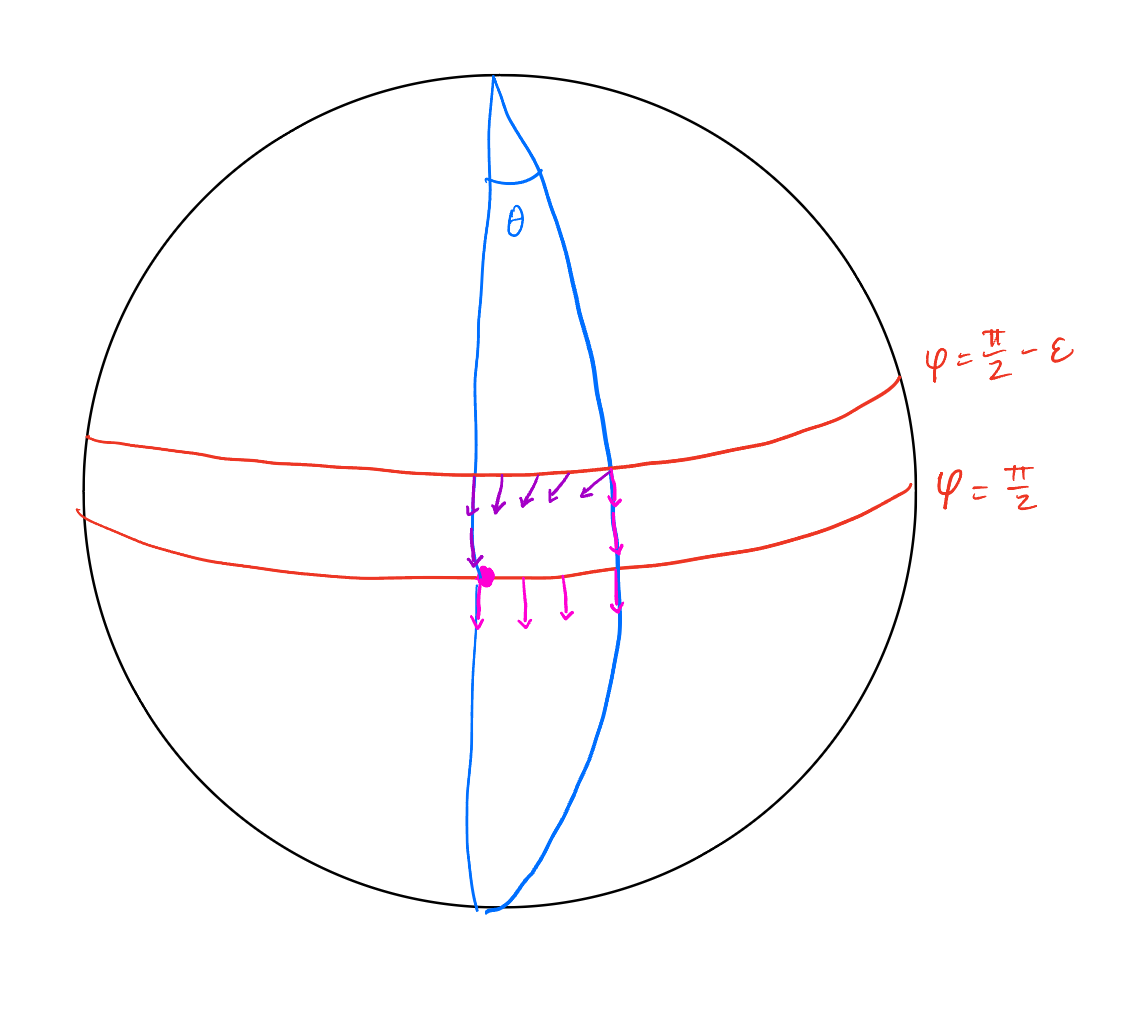
\includegraphics[scale=0.4]{transport.png}
\end{center}
Observe that parallel transport first up through a meridian and then along the latitude $\varphi=(\pi/2)-\epsilon$ (the route of purple vectors) yields a vector that is different from going the other route (the route of pink vectors) around the rectangle. The difference between the two resulting vectors is
\begin{equation}\label{eq1.0.15}
V(\theta)-(\partial_{\varphi})_{(\theta,(\pi/2)-\epsilon)}=-\frac{\sin{((\sin{\epsilon})\theta)}}{\cos{\epsilon}}(\partial_{\theta})_{(\theta,(\pi/2)-\epsilon)}+\left[\cos{((\sin{\epsilon})\theta)-1}\right](\partial_{\varphi})_{(\theta,(\pi/2)-\epsilon)}
\end{equation}
Writing out the terms to second order in $\epsilon$ and $\theta$, Equation \ref{eq1.0.15} becomes
\begin{equation}\label{eq1.0.16}
V(\theta)-(\partial_{\varphi})_{(\theta,(\pi/2)-\epsilon)}=-\epsilon\theta(\partial_{\theta})_{(\theta,(\pi/2)-\epsilon)}+O\left(\|(\epsilon,\theta)\|^3\right),
\end{equation}
but it is clear from our Christoffel symbols that
\begin{equation}
\begin{split}
R(\partial_{\theta},\partial_{\varphi})\partial_{\varphi}&=\nabla_{\partial_{\theta}}\nabla_{\partial_{\varphi}}\partial_{\varphi}-\nabla_{\partial_{\varphi}}\nabla_{\partial_{\theta}}\partial_{\varphi}\\
&=-\nabla_{\partial_{\varphi}}((\cot{\varphi})\partial_{\theta})\\
&=(-\cot^2{\varphi}+\csc^2{\varphi})\partial_{\theta}\\
&=-\partial_{\theta}.
\end{split}
\end{equation}
So actually Equation \ref{eq1.0.16} can be written as
\begin{equation}
V(\theta)-(\partial_{\varphi})_{(\theta,(\pi/2)-\epsilon)}=\epsilon\theta(R(\partial_{\theta},\partial_{\varphi})\partial_{\varphi})_{(\theta,(\pi/2)-\epsilon)}+O\left(\|(\epsilon,\theta)\|^3\right).
\end{equation}
This is the geometric essence of curvature. The curvature of the sphere is what causes parallel transport from one vertex of a coordinate rectangle to the opposite one along two different edge paths to yield different results. Our computation above shows that up to second order in the side lengths of the rectangle, the difference is reflected by the vector $(R(\partial_{\theta},\partial_{\varphi})\partial_{\varphi})_{(\theta,(\pi/2)-\epsilon)}$. This is a slight coincidence in our case as we will see in Theorem \ref{curvaturearea} that the correct difference vector up to second order is actually $(R(\partial_{\theta},\partial_{\varphi})\partial_{\varphi})_{(0,\pi/2)\to(\theta,(\pi/2)-\epsilon)}$, which is defined to be the parallel transport of $(R(\partial_{\theta},\partial_{\varphi})\partial_{\varphi})_{(0,\pi/2)}$ to $(\theta,(\pi/2)-\epsilon)$ along either edge path in the coordinate rectangle. In any case, we have sufficient probable cause to give $R$ a worthy name.

\begin{definition}
Let $M$ be a Riemannian manifold of dimension at least $2$ and let $\nabla$ be its Levi-Civita connection. The map $R\colon\mathfrak{X}(M)\times\mathfrak{X}(M)\times\mathfrak{X}(M)\to\mathfrak{X}(M)$ defined by
\begin{equation}
R(X,Y)Z\coloneqq\nabla_X\nabla_YZ-\nabla_Y\nabla_XZ-\nabla_{[X,Y]}Z
\end{equation}
is $C^{\infty}(M)$-linear in all three arguments and is thus a $(3,1)$-tensor field on $M$ called the \textbf{Riemann curvature tensor}.
\end{definition}

It is actually not obvious from the definition that $R$ is tensorial. In fact, the definition suggests the opposite as it alludes to covariant and Lie derivatives. It is a simple calculation using the Leibniz rule that the particular combination of derivatives in the definition of $R$ is nonetheless $C^{\infty}(M)$-trilinear and thus tensorial. This is also a motivation for the term $\nabla_{[X,Y]}Z$ in the definition. The upshot of tensoriality is that for any point $p\in M$, $R$ descends to a $\mathbb{R}$-trilinear map $R_p\colon T_p(M)\times T_p(M)\times T_p(M)\to T_p(M)$, which can be computed on tangent vectors $X_p$, $Y_p$, and $Z_p$ by just extending those vectors smoothly to vector fields, applying $R$, and then evaluating at $p$.

To establish our geometric interpretation of the Riemann curvature tensor, we first need the following technical lemma.

\begin{lemma}\label{paralleltransports}
Let $M$ be a smooth manifold of dimension at least $2$, and let $\nabla$ be a connection on $M$. Suppose $X$ and $Y$ are commuting vector fields in a neighborhood of $p\in M$, so that their flows $\Phi_X$ and $\Phi_Y$ form coordinate rectangles in the neighborhood. Let $S$ be a coordinate rectangle whose vertices are $p$, $p'\coloneqq\Phi_{X}^{p}(\epsilon)$, $q'\coloneqq\Phi_{Y}^{p}(\delta)$, and $q\coloneqq\Phi_X^{q'}(\epsilon)=\Phi_Y^{p'}(\delta)$ for some sufficiently small $\epsilon,\delta>0$.

Let $V\in T_p(M)$ be a tangent vector. Let $U\in T_q(M)$ be the parallel transport of $V$ along the sides of $S$ from $p$ to $p'$ to $q$, and let $W\in T_q(M)$ be the parallel transport of $V$ along the sides of $S$ from $p$ to $q'$ to $q$. Then relative to a coordinate frame containing $X$ and $Y$,
\begin{equation}
U_k=V_k-\epsilon V_j\Gamma_{X,j}^{k}(p)-\delta V_j\Gamma_{Y,j}^{k}(p)+\epsilon\delta\left(V_i\Gamma_{X,i}^{j}(p)\Gamma_{Y,j}^{k}(p)-V_jX(\Gamma_{Y,j}^k)|_p\right)+O(\epsilon^2,\delta^2),
\end{equation}
\begin{equation}
W_k=V_k-\delta V_j\Gamma_{Y,j}^{k}(p)-\epsilon V_j\Gamma_{X,j}^{k}(p)+\epsilon\delta\left(V_i\Gamma_{Y,i}^{j}(p)\Gamma_{X,j}^{k}(p)-V_jY(\Gamma_{X,j}^{k})|_p\right)+O(\epsilon^2,\delta^2).
\end{equation}
\end{lemma}

\begin{proof}
We will derive the formula for $U_k$. The formula for $W_k$ follows completely analogously.

Let $T$ be the parallel vector field on the edge from $p$ to $p'$ given by parallel transport of $V$. By Taylor's theorem and the parallel transport equation,
\begin{equation}\label{eq1.0.21}
T_k(\epsilon)=V_k+\epsilon T_k'(0)+O(\epsilon^2)=V_k-\epsilon V_j\Gamma_{X,j}^k(p)+O(\epsilon^2).
\end{equation}
Now let $Q$ be the parallel vector field on the edge from $p'$ to $q$ given by parallel transport of $T(\epsilon)$. By Taylor's theorem, the parallel transport equation, and Equation \ref{eq1.0.21},
\begin{equation}
\begin{split}
Q(\delta)_k&=T_k(\epsilon)+\delta Q_k'(0)+O(\delta^2)\\
&=V_k-\epsilon V_j\Gamma_{X,j}^k(p)-\delta\Gamma_{Y,j}^{k}(p')\left(V_j-\epsilon V_i\Gamma_{X,i}^{j}(p)\right)+O(\epsilon^2,\delta^2).
\end{split}
\end{equation}
The result now follows from combining this with Taylor's theorem applied to $\Gamma_{Y,j}^k$, which tells us that
\begin{equation}
\Gamma_{Y,j}^k(p')=\Gamma_{Y,j}^k(p)+\epsilon X(\Gamma_{Y,j}^k)|_p+O(\epsilon^2).
\end{equation}
\end{proof}

We can now state and prove our result which gives us a geometric interpretation of the Riemann curvature tensor.

\begin{theorem}\label{curvaturearea}
Let $M$ be a Riemannian manifold of dimension at least $2$, and let $R$ be the Riemann curvature tensor on $M$. Suppose $X$ and $Y$ are commuting vector fields in a neighborhood of $p\in M$, so that their flows $\Phi_X$ and $\Phi_Y$ form coordinate rectangles in the neighborhood. Let $S$ be a coordinate rectangle whose vertices are $p$, $p'\coloneqq\Phi_{X}^{p}(\epsilon)$, $q'\coloneqq\Phi_{Y}^{p}(\delta)$, and $q\coloneqq\Phi_X^{q'}(\epsilon)=\Phi_Y^{p'}(\delta)$ for some sufficiently small $\epsilon,\delta>0$.

Let $V\in T_p(M)$ be a tangent vector. Let $U\in T_q(M)$ be the parallel transport of $V$ along the sides of $S$ from $p$ to $p'$ to $q$, and let $W\in T_q(M)$ be the parallel transport of $V$ along the sides of $S$ from $p$ to $q'$ to $q$. Let $(R_p(X_p,Y_p)V)_{p\to q}$ be the parallel transport of $R_p(X_p,Y_p)V\in T_p(M)$ to $q$ along either edge path of $S$. Then,
\begin{equation}\label{eq1.0.25}
W-U=\epsilon\delta(R_p(X_p,Y_p)V)_{p\to q}+O\left(\|(\epsilon,\delta)\|^3\right).
\end{equation}
\end{theorem}

\begin{proof}
We first calculate the components of $R_p(X_p,Y_p)V$. Since the curvature tensor is defined in terms of derivatives, we must extend $V$ to a smooth vector field, which we call $\tilde{V}$, to first calculate $R(X,Y)\tilde{V}$. As predicted by tensoriality, we will see that all derivatives of $\tilde{V}$ cancel which means the result will only depend on the vector $V\in T_p(M)$, and not on our choice of extension to a vector field. We use the Einstein summation convention which means all indices in the following calculation (except the fixed index $k$) are implicitly being summed over.
\begin{equation}\label{eq1.0.26}
\begin{split}
(R(X,Y)\tilde{V})_k&=\nabla_X\nabla_Y\tilde{V}-\nabla_Y\nabla_X\tilde{V}\\
&=\nabla_X\left[(Y_i\partial_i(\tilde{V}_{\alpha})+Y_i\tilde{V}_j\Gamma_{i,j}^{\alpha})\partial_{\alpha}\right]-\nabla_Y\left[(X_i\partial_i(\tilde{V}_{\alpha})+X_i\tilde{V}_j\Gamma_{i,j}^{\alpha})\partial_{\alpha}\right]\\
&=X_i\partial_i\left(Y_m\partial_m(\tilde{V}_k)+Y_m\tilde{V}_{\ell}\Gamma_{m,\ell}^{k}\right)+X_i\left(Y_m\partial_m(\tilde{V}_j)+Y_m\tilde{V}_{\ell}\Gamma_{m,\ell}^{j}\right)\Gamma_{i,j}^{k}\\
&\phantom{{}={}}-Y_i\partial_i\left(X_m\partial_m(\tilde{V}_k)+X_m\tilde{V}_{\ell}\Gamma_{m,\ell}^{k}\right)-Y_i\left(X_m\partial_m(\tilde{V}_j)+X_m\tilde{V}_{\ell}\Gamma_{m,\ell}^{j}\right)\Gamma_{i,j}^k\\
&=\partial_X\left(\partial_Y(\tilde{V}_k)+\tilde{V}_{\ell}\Gamma_{Y,\ell}^{k}\right)+\left(\partial_Y(\tilde{V}_j)+\tilde{V}_{\ell}\Gamma_{Y,\ell}^{j}\right)\Gamma_{X,j}^{k}\\
&\phantom{{}={}}-\partial_Y\left(\partial_X(\tilde{V}_k)+\tilde{V}_{\ell}\Gamma_{X,\ell}^{k}\right)-\left(\partial_X(\tilde{V}_j)+\tilde{V}_{\ell}\Gamma_{X,\ell}^{j}\right)\Gamma_{Y,j}^{k}\\
&=\partial_{X}(\tilde{V}_{\ell}\Gamma_{Y,\ell}^{k})+\partial_{Y}(\tilde{V}_j)\Gamma_{X,j}^{k}+\tilde{V}_{\ell}\Gamma_{Y,\ell}^{j}\Gamma_{X,j}^k-\partial_{Y}(\tilde{V}_{\ell}\Gamma_{X,\ell}^{k})-\partial_X(\tilde{V}_j)\Gamma_{Y,j}^k-\tilde{V}_{\ell}\Gamma_{X,\ell}^{k}\Gamma_{Y,j}^{k}\\
&=\tilde{V}_jX(\Gamma_{Y,j}^k)-\tilde{V}_jY(\Gamma_{X,j}^k)+\tilde{V}_i\Gamma_{Y,i}^{j}\Gamma_{X,j}^{k}-\tilde{V}_i\Gamma_{X,i}^{j}\Gamma_{Y,j}^{k}.
\end{split}
\end{equation}
The first equality is because $[X,Y]=0$, the fourth equality comes from the fact that we are working in a coordinate frame containing $X$ and $Y$, the fifth equality uses Clairaut's theorem to cancel some terms, and the last equality comes from the Leibniz rule. As claimed there are no derivatives left in the final expression, so we may evaluate it freely at $p$.

Applying Lemma \ref{paralleltransports} to the Levi-Civita connection on $M$, we obtain formulas for the components of $U$ and $W$. When we subtract those formulas, all terms up to first order cancel leaving behind
\begin{equation}\label{eq1.0.27}
W_k-U_k=\epsilon\delta\left(V_jX(\Gamma_{Y,j}^k)|_p-V_jY(\Gamma_{X,j}^k)|_p+V_i\Gamma_{Y,i}^{j}(p)\Gamma_{X,j}^{k}(p)-V_i\Gamma_{X,i}^{j}(p)\Gamma_{Y,j}^{k}(p)\right)+O(\epsilon^2,\delta^2).
\end{equation}
Notice that if we take either $\epsilon\to0$ or $\delta\to0$, the rectangle should collapse so that both edge paths become the same and thus $W_k=U_k$. Hence for any power $n$, there cannot be any pure $\epsilon^n$ or $\delta^n$ terms in Equation \ref{eq1.0.27}, for such terms would represent an obstruction to the vanishing of $W_k-U_k$ when $\delta=0$ or $\epsilon=0$, respectively. In particular, there are no $\epsilon^2$ or $\delta^2$ terms so the error term $O(\epsilon^2,\delta^2)$ in Equation \ref{eq1.0.27} can be improved to order $3$:
\begin{equation}\label{eq1.0.28}
W_k-U_k=\epsilon\delta\left(V_jX(\Gamma_{Y,j}^k)|_p-V_jY(\Gamma_{X,j}^k)|_p+V_i\Gamma_{Y,i}^{j}(p)\Gamma_{X,j}^{k}(p)-V_i\Gamma_{X,i}^{j}(p)\Gamma_{Y,j}^{k}(p)\right)+O\left(\|(\epsilon,\delta)\|^3\right).
\end{equation}
Now we observe that by Equation \ref{eq1.0.26}, the $\epsilon\delta$ term above is precisely the $k$\textsuperscript{th} component of $R_p(X_p,Y_p)V$. Therefore,
\begin{equation}\label{eq1.0.29}
W_k-U_k=\epsilon\delta(R_p(X_p,Y_p)V)_k+O\left(\|(\epsilon,\delta)\|^3\right).
\end{equation}
By Lemma \ref{paralleltransports} applied to $R_p(X_p,Y_p)V\in T_p(M)$, the components of $(R_p(X_p,Y_p)V)_{p\to q}$ agree with the components of $R_p(X_p,Y_p)V$ itself up to zeroth order regardless of our choice of edge path from $p$ to $q$. Since $\epsilon\delta$ is quadratic, it follows that $W-U-\epsilon\delta(R_p(X_p,Y_p)V)_{p\to q}$ is cubic in $\epsilon$ and $\delta$ and this establishes Equation \ref{eq1.0.25}.
\end{proof}


\end{section}

\begin{section}{Formal Properties of the Curvature Tensor}
In this section we will begin the consideration of arbitrary connections on general vector bundles. Just as the Riemann curvature tensor is defined from the Levi-Civita connection, arbitrary connections will give rise to curvature tensors.

\begin{definition}
Let $M$ be a smooth manifold and let $(E,\pi\colon E\to M)$ be a vector bundle on $M$. Let $\nabla\colon\mathfrak{X}(M)\times\Gamma(M,E)\to\Gamma(M,E)$ be a connection on $E$. Let $e_1,\dots,e_r$ be a local frame for $E$. Then there are $1$-forms $\omega_j^i$, defined in the neighborhood of the local frame, such that
\begin{equation}\label{eq2.0.1}
\nabla_Xe_j=\sum_i{\omega_j^i(X)e_i}
\end{equation}
for all vector fields $X$. These $\omega_j^i$ are called the \textbf{connection forms} of $\nabla$ relative to the frame $e_1,\dots,e_r$.
\end{definition}

Observe that the connection forms do not transform tensorially upon choosing a different local frame, so they are not intrinsic invariants of the connection, though this fact is somewhat suppressed in the notation. The motivating example is when $\nabla$ is a linear connection, in which case the connection $1$-forms are essentially the Christoffel symbols since $\Gamma_{i,j}^k=\omega_j^k(e_i)$.

\begin{definition}
Let $M$ be a smooth manifold and let $\nabla$ be a linear connection on $M$. The map $\tau\colon\mathfrak{X}(M)\times\mathfrak{X}(M)\to\mathfrak{X}(M)$ defined by
\begin{equation}\label{eq2.0.2}
\tau(X,Y)\coloneqq \nabla_{X}Y-\nabla_{Y}X-[X,Y]
\end{equation}
is a $(2,1)$-tensor field on $M$ called the \textbf{torsion tensor} of $\nabla$.
\end{definition}

Observe that this tensor is what needs to vanish in part of the definition of the Levi-Civita connection. In general, we have the following relationship between the connection forms of a linear connection and the torsion tensor.

\begin{theorem}[Cartan's First Structure Equation]
Let $M$ be a smooth manifold and let $\nabla$ be a linear connection on $M$. Suppose we work relative to the local frame $e_1,\dots,e_n$ with dual coframe $\varphi^1,\dots,\varphi^n$. Then relative to these frames,
\begin{equation}\label{eq2.0.3}
d\varphi^j=\tau^j+\sum_{i}{(\varphi^i\wedge\omega_i^j)}.
\end{equation}
\end{theorem}
\end{section}


\clearpage

\bibliographystyle{plain}
\bibliography{bibliography}


\end{document}